\documentclass{amsart}
\usepackage{graphicx}
\graphicspath{{./}}
\usepackage{hyperref}
\usepackage{csvsimple}
\usepackage{longtable}
\usepackage{lscape}
\usepackage{epigraph}
\title{Difference Between the Project of Adolphe Quetelet 1796-1874 And Mine}
\author{Zulfikar Moinuddin Ahmed}
\date{\today}
\begin{document}
\maketitle

\section{Adolphe Quetelet's Social Physics}

Quetelet worked in astronomy, and he wanted to apply the methods of statistical analysis to produce accounts of regularity for Human Beings.  

First of all, I confess that I discovered Quetelet yesterday for the first time from examining the {\em History of Statistics} of Stigler and did not know about him at all.  But I immediately recognised him as a kindred spirit.  I had turned towards Human Personality Psychology and Human Nature problems since my great success in overthrowning Relativity, Schroedinger's Quantum Theory, and Expansionary Cosmology in 2018, and gained confidence since Freeman Dyson said I was right.  

Unlike Quetelet, I do not believe that it will be easy to establish a sharp Social Science without a tremendous amount of deeper understanding about the relationship between our scientific theories and Nature.  

I will give an example of the sort of thing I mean.  You see Empiricism is easy with Physics and Physical Chemistry because even with the deep complexity of these subjects, there are infinitely easier issues of statistical inference from data.  Our Physics and Physical Chemistry theories have evolved enough that the concepts employed are close to Nature's actual functioning; Four-Sphere Theory is close to being Absolute Truth.

In contrast, there are many deep and difficult issues of statistical inference in Social Sciences whose maturity is quite a bit more imperfect and so there is a fundamental question always of whether Nature {\em respects} the concepts being measured.  In other words, when we measure the charge of an electron, our experience has shown persistence of these measurements for a century or more.  So assuming that our notion of 'charge' is Nature's notion something existential about Nature, is reasonable.  In Social Sciences, not a single variable can claim this association.  Most Social Science variables are not plasibly fundamental to Nature.  They are all creative inventions of human individuals, and there is not enough justification to consider any of them to have the blessings of Nature at all.  This is why psychology perpetually is grappling with estimates of reliability of construct in measurements.

For myself, this is not a failing of Social Science at all.  It bespeaks of enormous positive {\em ambition} of Social Scientists compared to Physicists.  But here we have a serious problem.  Often the scale of the scientific ambition is not matched by sufficiently strong intellectual infrastructure for statistical inference.  Often there is more effort in statistical inference in {\em Physics} where there are relatively fewer difficulties, and less effort in Social Sciences, which actually need a great deal more effort because the variables are wobblier.

\section{I Have Proven Regularity In Human Nature Far Deeper Than Quetelet}

I want to be quite clear that I have proven regularity in Human Nature far deeper than Adolphe Quetelet had in his lifetime.  I have proven ethnicity-independent regularity in moral values, in life preferences, and childrearing values across human race.  Quetelet had not done any of this during his lifetime.

I want this to be clear. I  was not a follower of Quetelet in {\em seeking regularity}.  Indeed, I slowly came to know the evidence for a Single Human Race over the past decade and was completely unaware of the work of Adolphe Quetelet some centuries ago.  

At the same time, once I did become aware of his work, I can give him credit for prefiguring the concept of human race regularities.  I focused on moral values, childrearing values, life preferences, and he focused on other sorts of regularities.  He must be acknowledged in his pioneering efforts, with others like Thomas Payne and Thomas Jefferson and other universalist theories.  I acknowledge their priority for universalism but I am the great genius who showed the regularity in morals with the high quality data of World Values Survey.  Quetelet simply did not have access to such global data at all and therefore was not able to establish truth of a Single Human Race and Quantitative Human Nature.

\section{Quetelet Pioneered Careful Fitting of Parametric Errors}

Much more than Francis Galton, it was Quetelet who began to fit binomial distributions to social measurements carefully.  Now it is a routine matter than binomial distributions approximate normal distribution, mentioned in the first chapter of Michel Louve's {\em Probability Theory} and other standard texts.  But in fact for Social Data he was one of the great pioneers.  I began doing this more than a year ago with Generalised Hyperbolic Distributions, and I have Finance Quant experience from Lehman Brothers from 1995.  But I have to give great credit to Quetelet for doing this in the nineteenth century, more than a century before I was even born.  His idea was right, that one ought to carefully match the exact distribution, but it would be a century after his death that the right parametric densities were discovered by Ole Barndorff-Nielsen in mid 1970s, so he was not doing this with the right parametric densities.  

\section{Study of Confidence in Church By Ethnicity}

I want to clear up some of my major scientific goals before I present results.  One of major hypotheses is that the {\em infinite possible variability} a priori in human race level statistics can be tamed exactly by Generalised Hyperbolic Distributions which are five parameter distributions.  This is great scientific progress.  In {\em theory} any variable measured across 7.8 billion people could produce arbitrary complexity in the profiles.  To make things clear, suppose the variable $v$ has ordered 10 levels.  Then a priori, in order to accurately model the totality of possible outcomes, we would need a 10 parameter model.  My claim is that in fact if we use GHD then for {\em every single frequency distribution} 5 parameter model will suffice to the edge of accuracy.  This is a serious hypothesis about all Social Science variables.  They all will satisfy this.  This is one of my major hypotheses, and I have already shown that it is true in some cases.  Below I will show more cases where GHD captures variable outcomes successfully.

I am very close to 100\% zealous in my conviction that Generalised Hyperbolic Distributions are deep discoveries of the nature of noise in the actual universe, that O. Barndorff-Nielsen has found the secret miracle of all Noise in Nature that will forever displace Gaussians as models of Noise.  

The second issue on my mind is the issue of universality of Human Nature.  Here I will show you an interesting subtle example.  Here Indians and Arabs behave in a different manner than the rest -- Whites, Blacks, East Asians, Others.  Here we are dealing with a variable that is {\em not Human Nature driven}.  

\section{Fits of GHD}

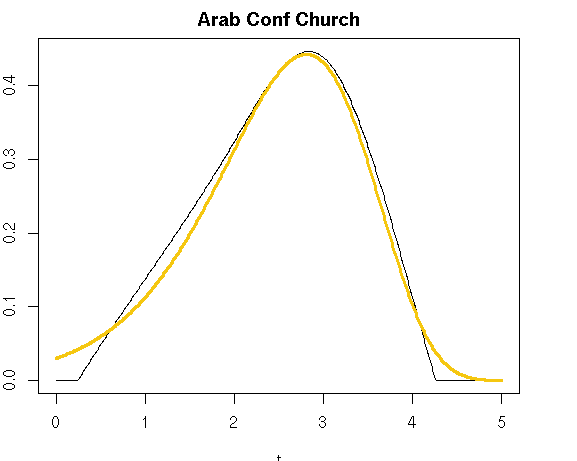
\includegraphics[scale=0.8]{cfchurch_arab.png}

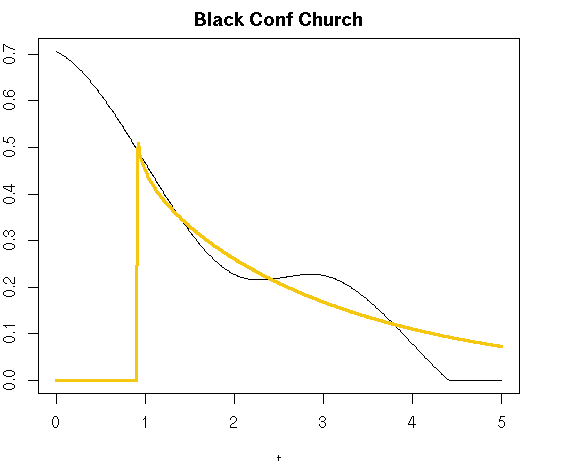
\includegraphics[scale=0.8]{cfchurch_black.png}

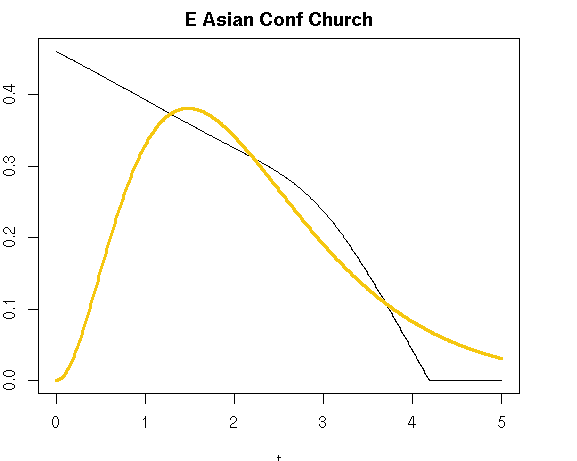
\includegraphics[scale=0.8]{cfchurch_eastasian.png}

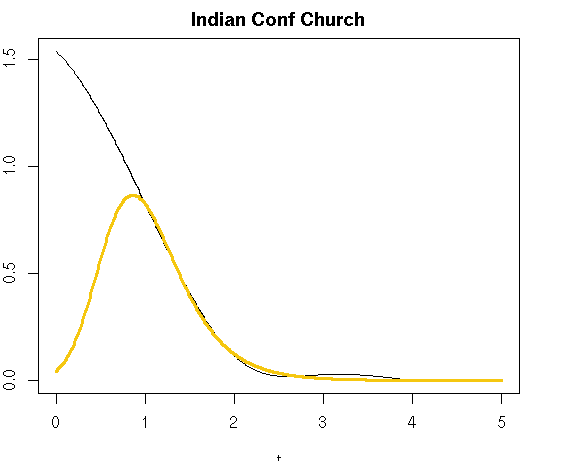
\includegraphics[scale=0.8]{cfchurch_indian.png}

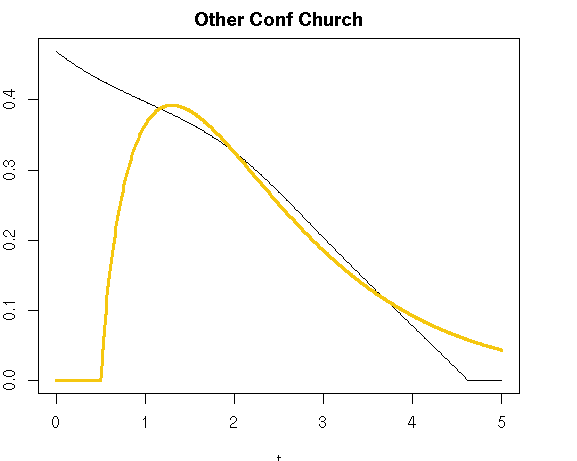
\includegraphics[scale=0.8]{cfchurch_other.png}

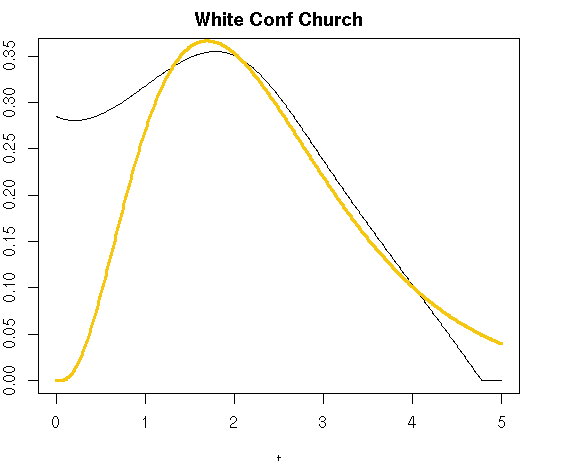
\includegraphics[scale=0.8]{cfchurch_white.png}

Now let's take a look at all the raw curves.

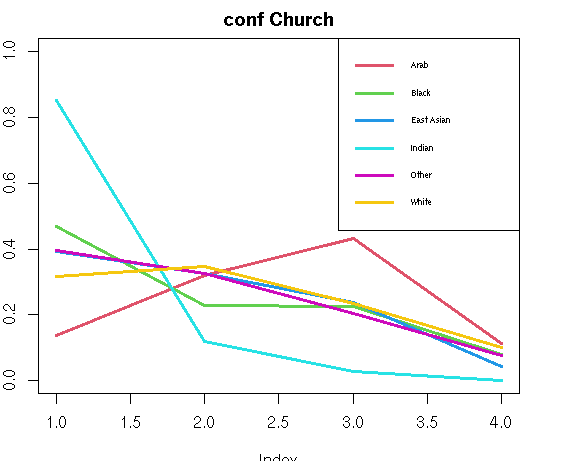
\includegraphics[scale=0.8]{cfchurch_raw.png}

Visually we can immediately pick out that there is a closeness of all other curves except Arabs and Indians.  So we want to just consider how to formalize this in statistical summary.  Here are the plot of the fitted GHD curves.

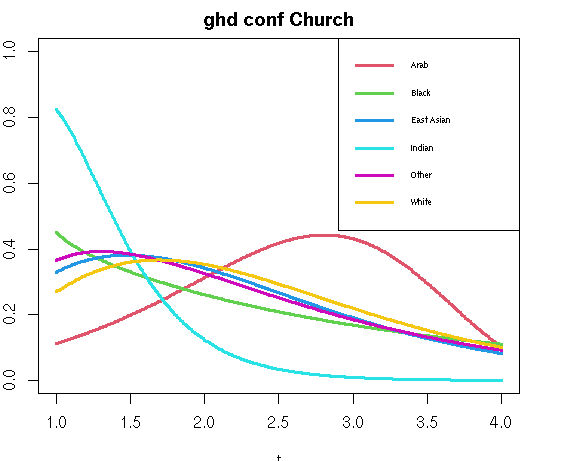
\includegraphics[scale=0.8]{cfchurch_ghd.png}

Let us now consider the fitted values to understand what is different about Indians and Arabs from the others.

% latex table generated in R 4.0.3 by xtable 1.8-4 package
% Mon May 17 21:14:24 2021
\begin{table}[ht]
\centering
\begin{tabular}{rlrrrrr}
  \hline
 & eth & lambda & mu & sigma & gamma & alpha.bar \\ 
  \hline
1 & Arab & -17.09 & 6.90 & 0.00 & -4.47 & 13.13 \\ 
  2 & Black & 0.94 & 0.91 & 0.00 & 2.37 & 0.03 \\ 
  3 & East Asian & 3.17 & 0.00 & 0.10 & 2.16 & 0.10 \\ 
  4 & Indian & -7.89 & 0.00 & 0.36 & 1.04 & 4.27 \\ 
  5 & Other & 1.75 & 0.51 & 0.00 & 1.85 & 0.02 \\ 
  6 & White & 3.48 & 0.04 & 0.05 & 2.32 & 0.00 \\ 
   \hline
\end{tabular}
\end{table}

I won't go through the analysis from here since it's standard after this point.

\section{The Key Points}

Our fitting is remarkably successful for all the curves, and the estimated parameters seem reasonable and allow us to produce good inferences about uniformity and effect of ethnicity.

\section{Consider Quetelet}

It was not a lack of talent and good ideas that led Quetelet to fail in a sense in his project.  His ideas were good, but he was simply born in the wrong century.  He will fall into the tragic man ahead of his times.  His project is much more possible to solve now thanks to advances of work on Levy Processes and the fabulous discovery of GHD by Ole Barndorff-Nielsen in 1976.  

In Science, many great problems have this character.  When I worked on Four-Sphere Theory, I paid a great deal of attention to alternative interpretations of Michelson-Morley given known the 1959 discovery of reality of EM potential.  And that produced a great success.  

Sometimes people have a theory of linear progress, and are competing in the cutting edge in various ways.  But Science is all of Nature, and for me, it is always worthwhile to take a grand historical perspective, for there are many problems that were impossible at different times and only a century later, only two centuries later, one sees what the real difficulty was, that the talented and enterprising scientific genius was born in the wrong century for what he or she needed.  

\section{Code}

\begin{verbatim}
stack.plot<-function( A, title, position="topleft", t=NULL){
  if (is.null(t)){
    t<-1:dim(A)[2]
  }
  par(mar=c(3.5,2,2,3))
  q<-plot(t, A[1,], type='l',lwd=3,ylim=c(0,1.0), col=1+1, main=title)
  n<-dim(A)[1]
  for ( j in 2:n){
    lines(t,A[j,], lwd=3, col=j+1)
  }
  legend(position,legend=row.names(A),col=seq(2,1+n),lwd=3,
         cex=0.5)
  q
}

g<-function( theta ){
  lambda<-theta[1]
  mu <- theta[2]
  sigma <- theta[3]
  gamma <- theta[4]
  alpha.bar <- theta[5]
  out <- ghyp( lambda=lambda,mu=mu,sigma=sigma,
               gamma=gamma,alpha.bar=alpha.bar)
  out
}

fit_ghd_shape<-function( t, z0 ){
  delta <- t[2]-t[1]
  eps<-1e-6
  z<-cubicspline(1:length(z0),z0,xi=t)
  z[z<eps]<-eps
  z<-z/(sum(z[t>0.5 & t<4.5])*delta)
  y<-z
  objective<-function( theta ){
    yp <- dghyp( t, object=g(theta))
    out<-sum( delta*(y[t>0.9 & t<4.3]- yp[t>0.9 & t < 4.3])^2)
    if (is.na(out)){
      print(theta)
      print(yp)    
    }
    out
  }
  theta0 <-c(-3.0,3.5,1.1,0.0,1.0)
  lower0<-c(-Inf,0,0.001,-Inf,0)
  upper0<-c(Inf,100,Inf,Inf,Inf)
  res<-optim( theta0, fn=objective,
              lower=lower0,
              upper=upper0,
              method="L-BFGS-B",control=list(trace=1,maxit=5000))
  
  yp<-dghyp( t, object=g(res$par))
  list(theta=res$par,t=t,x=z,y=yp)
}

\end{verbatim}
  
  


\end{document}